\documentclass[
  tikz, convert={density=800, size = 2400x2400},
  border=0.5cm
]{standalone}
\usepackage{amsmath, amssymb, amsthm, bm, bbm, xcolor}

\usetikzlibrary{shapes.geometric, positioning}
\usetikzlibrary{quotes, angles, calc, backgrounds}
\definecolor{BadgerRed}{cmyk}{0.03, 1, 0.66, 0.12}

\definecolor{myColor1}{RGB}{153,153,153}
\definecolor{myColor2}{RGB}{230,159,0}
\definecolor{myColor3}{RGB}{86,180,233}
\definecolor{myColor4}{RGB}{0,158,115}
\definecolor{myColor5}{RGB}{240,228,66}
\definecolor{myColor6}{RGB}{0,114,178}
\definecolor{myColor7}{RGB}{213,94,0}
\definecolor{myColor8}{RGB}{204,121,167}

\tikzset{decisionNode/.style={inner sep=7pt, shape=circle,align=center,font=\Huge,draw, fill=white}}
\tikzset{leafNode/.style={inner sep=7pt, shape=circle, align=center, font = \Huge, draw, fill=white}}
\tikzset{decisionRule/.style={shape=rectangle, align=center, font = \normalsize, draw=none, fill=white}}
\tikzset{jump/.style={shape=rectangle, align=center, font=\Large, draw=none, fill=white}}
\tikzset{annotation/.style={shape=rectangle, align=center, font=\Large, draw=none, fill=white}}

\begin{document}
\def\P{\mathbb{P}}
\def\bx{\bm{x}}

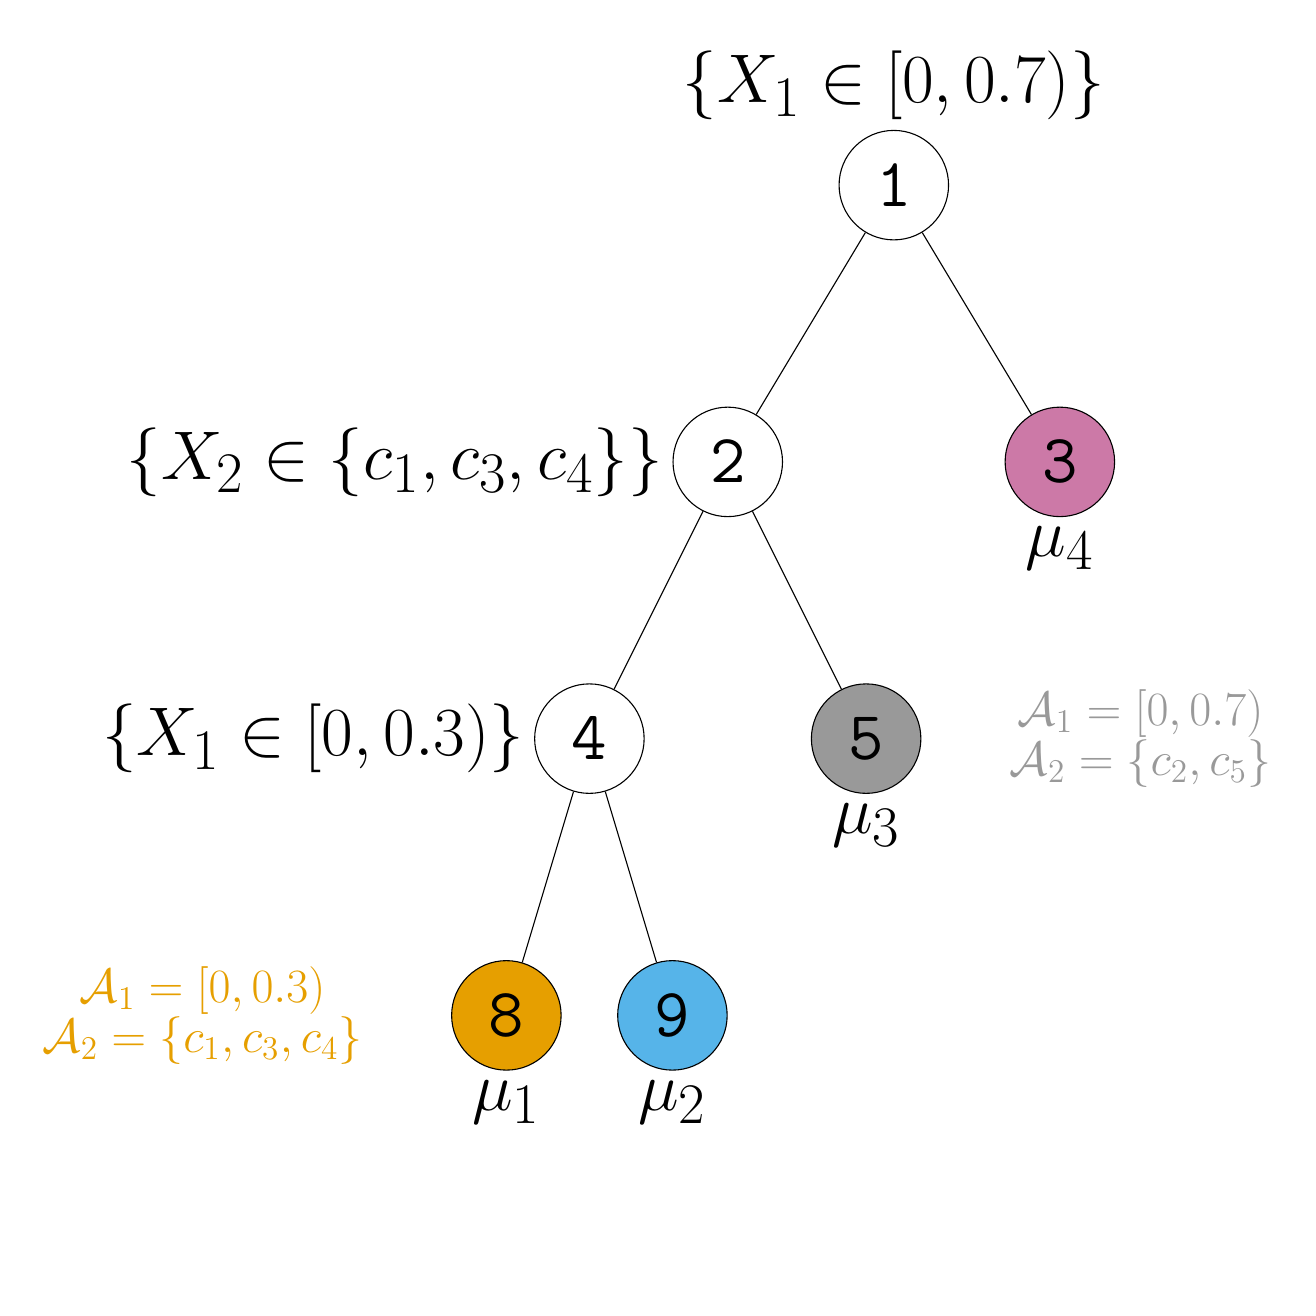
\begin{tikzpicture}[
  background rectangle/.style={fill=white}, show background rectangle,
  level 1/.style={sibling distance = 12em},
  level 2/.style={sibling distance = 10em},
  level 3/.style={sibling distance = 6em},
  level 4/.style={sibling distance = 5em},
  level distance = 10em]

\useasboundingbox (-8,-8) rectangle (8,8);

%, label=above:{\Huge $\textcolor{BadgerRed}{$D_{1}$}}
\node[decisionNode, label=above:{\Huge $\{X_{1} \in [0,0.7)\}$}]  (1) at (3,6) {\texttt{1}}
  child{ % 2 and its children
    node[decisionNode, label=left:{\Huge $\{X_{2} \in \{c_{1}, c_{3}, c_{4}\}\}$}] (2) {\texttt{2}}
      child{ % 4 and its children
        node[decisionNode, label = left:{\Huge $\{X_{1} \in [0,0.3)\}$}] (4) {\texttt{4}}
          child{ node[leafNode, label=below:{\Huge $\mu_{1}$}, fill = myColor2] (8) {\texttt{8}}}
          child{ node[leafNode, label=below:{\Huge $\mu_{2}$}, fill = myColor3] (9) {\texttt{9}} }
      }
      child{node[leafNode, label=below:{\Huge $\mu_{3}$}, fill = myColor1] (5) {\texttt{5}}}
  }
  child{node[leafNode, label=below:{\Huge $\mu_{4}$}, fill = myColor8] (3) {\texttt{3}}}
;


\draw node[annotation, left=of 8]{ \textcolor{myColor2}{\LARGE $\mathcal{A}_{1} = [0, 0.3)$} \\ \textcolor{myColor2}{\LARGE $\mathcal{A}_{2} = \{c_{1}, c_{3}, c_{4}\}$} };
\draw node[annotation, right=of 5]{ \textcolor{myColor1}{\LARGE $\mathcal{A}_{1} = [0, 0.7)$} \\ \textcolor{myColor1}{\LARGE $\mathcal{A}_{2} = \{c_{2}, c_{5}\}$}};
%\draw node[annotation, right=of 9] {$\mathcal{A}(1) = [0.3, 0.7)$ \\ $\mathcal{A}(2) = \{c_{1}, c_{3}, c_{4}\}$};
%\draw (1) edge[auto=right,pos=0.5,"\Huge$X_{1} < 0.7$"] (2);
%\draw (1) edge[auto=left,pos=0.5,"\Huge$X_{1} \geq 0.7$"] (3);

%\draw (2) edge[auto=right, pos=0.65, "\Huge$X_{2} < 0.6$"] (4);
%\draw (2) edge[auto=left, pos=0.65,"\Huge$X_{2} \geq 0.6$"] (5);

%\draw (4) edge[auto=right, pos=0.75, "\Huge$X_{1} < 0.3$"] (8);
%\draw (4) edge[auto=left, pos=0.75, "\Huge$X_{1} \geq 0.3$"] (9);

\end{tikzpicture}

\end{document}